\section{Denavit-Hartenberg Formulation}
\label{sec:dh}

{\renewcommand{\arraystretch}{1.2}
\begin{table}[t]
    \caption{DH Table for minibot-7R}
    \label{tab:dh}
    \centering
    \begin{tabular}{ *5l }           \toprule
      \emph{Link}  & \emph{$\alpha_i$} [\unit{\degree}]& \emph{$a_i$} & \emph{$d_i$}\; [\unit{\milli\meter}] & \emph{$\theta_i$} [\unit{\degree}]\\ 
      \cmidrule(lr){1-1} \cmidrule(lr){2-2} \cmidrule(lr){3-3} \cmidrule(lr){4-4} \cmidrule(lr){5-5}
      $1$ & $90$ & $0$ & $-450.5$ & $\theta_1^*$ \\
    $2$ & $-90$ & $0$ & $0$ & $\theta_2^*$ \\
    $3$ & $90$ & $0$  & $-320.5$ & $\theta_3^*$ \\
    $4$ & $-90$ & $0$ & $0$ & $\theta_4^*$ \\
    $5$ & $-90$ & $0$ & $-256$ & $\theta_5^*$ \\
    $6$ & $90$ & $0$ & $0$ & $\theta_6^*$ \\
    $7$ & $0$ & $0$ & $-106$ & $\theta_7^*$ \\ \midrule
    Home: & $\theta_i = 0^\circ$, & $i \neq 4$; & & $\theta_4 = 90^\circ$ \\
    \bottomrule
    \hline
    \end{tabular}
\end{table}
}

The transformation matrices between consecutive frames are given as follows.

\begin{align}
  \begin{split}
    A_1 &= \bmat{ c_1 & 0 & s_1 & 0 \\ s_1 & 0 & -c_1 & 0 \\ 0 & 1 & 0 & d_1 \\ 0 & 0 & 0 & 1}, \;\;
    A_2 = \bmat{ c_2 & 0 & -s_2 & 0 \\ s_2 & 0 & c_2 & 0 \\ 0 & -1 & 0 & 0 \\ 0 & 0 & 0 & 1}, \\
    A_3 &= \bmat{ c_3 & 0 & s_3 & 0 \\ s_3 & 0 & -c_3 & 0 \\ 0 & 1 & 0 & d_3 \\ 0 & 0 & 0 & 1}, \;\;
    A_4 = \bmat{ c_4 & 0 & -s_4 & 0 \\ s_4 & 0 & c_4 & 0 \\ 0 & -1 & 0 & 0 \\ 0 & 0 & 0 & 1}, \\
    A_5 &= \bmat{ c_5 & 0 & -s_5 & 0 \\ s_5 & 0 & c_5 & 0 \\ 0 & -1 & 0 & d_5 \\ 0 & 0 & 0 & 1}, \;\;
    A_6 = \bmat{ c_6 & 0 & s_6 & 0 \\ s_6 & 0 & -c_6 & 0 \\ 0 & 1 & 0 & 0 \\ 0 & 0 & 0 & 1}, \\
    A_7 &= \bmat{ c_7 & -s_7 & 0 & 0 \\ s_7 & c_7 & 0 & 0 \\ 0 & 0 & 1 & d_7 \\ 0 & 0 & 0 & 1}. \\
  \end{split}
\end{align}
%
The forward kinematics map is then given by \[ f: \mc{Q} \triangleq \prod_1^7
\mathbb{S}^1 \rightarrow \SEthree, \quad f(\bm{q}) = \prod_1^7 A_i(\theta_i), \]
%
% where $q_i = \theta_i$ are the joint variables.

% An alternative assignment of frames is shown in Figure~\ref{fig:minibot_alt}
% %
% \begin{figure}[h]
%   \centering
%   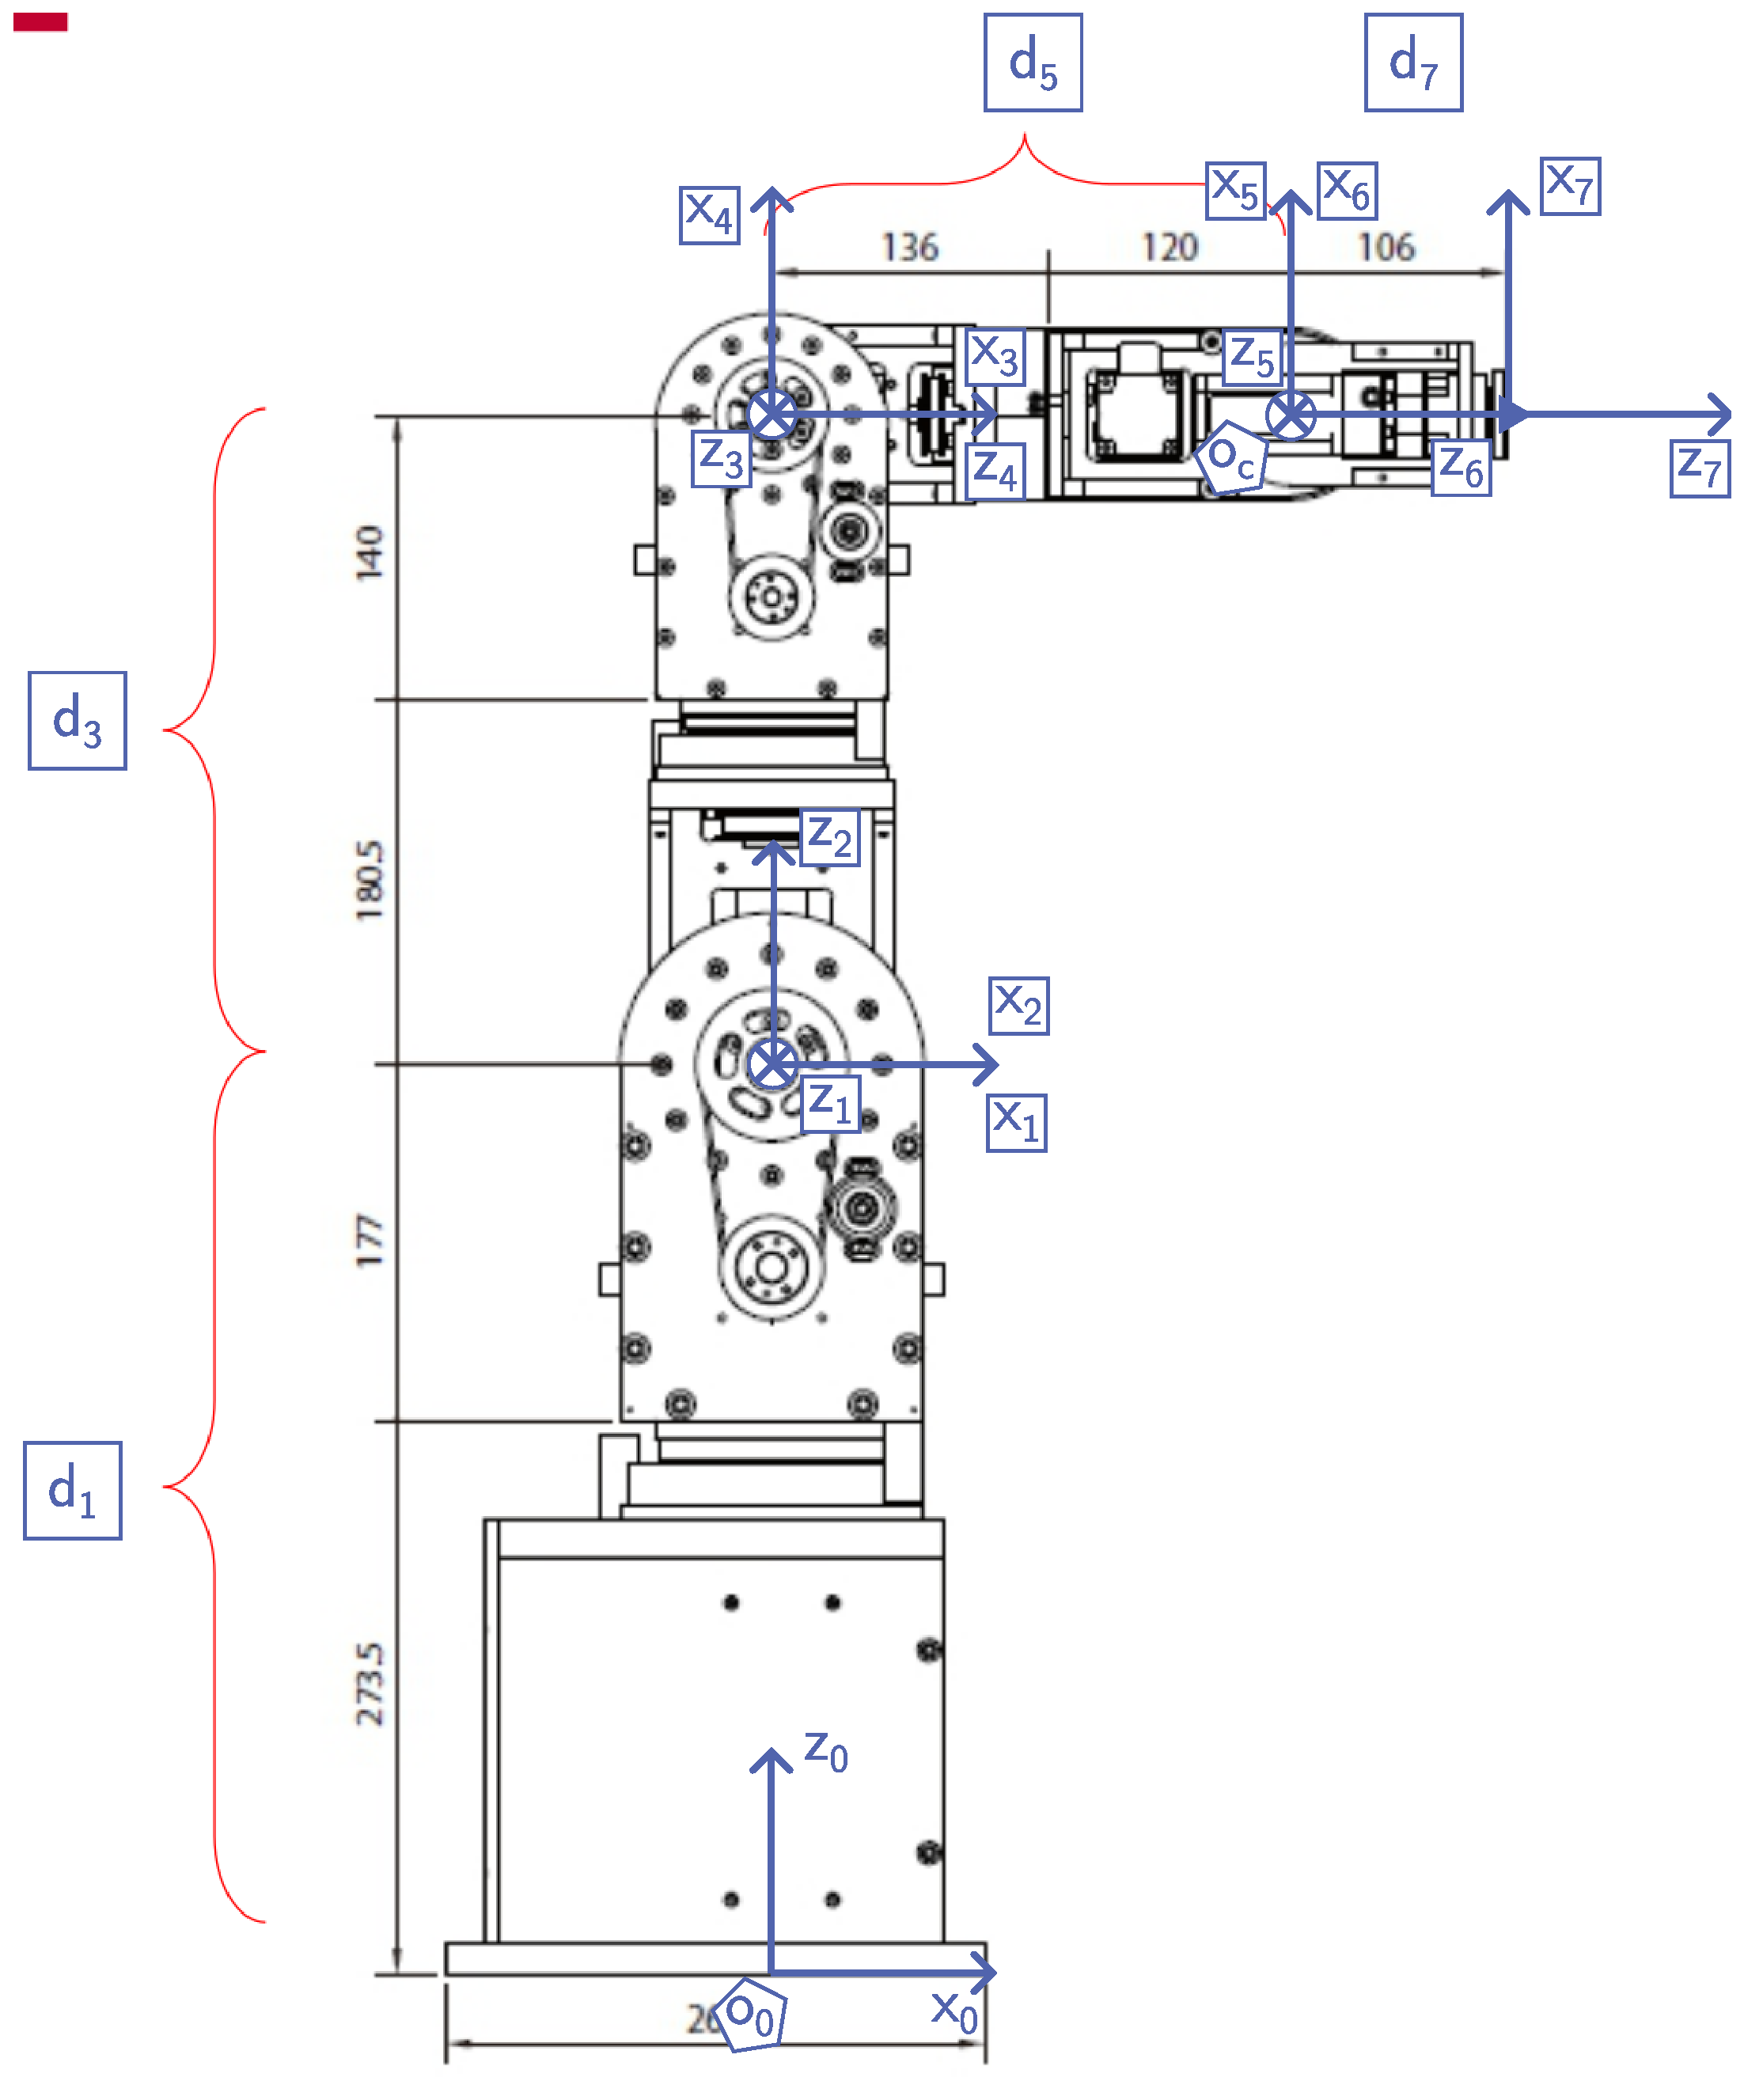
\includegraphics[width=0.5\textwidth]{./figures/minibot-7R_alternative.eps}
%   \caption{Schematic of minibot-7R: Alternative DH frame assignment.}
%   \label{fig:minibot_alt}
% \end{figure}
% %
% When the frames are assigned in this way, the DH table~\ref{tab:dh} still
% remains valid, except for the fact that the fact that at home position, we now
% have $\theta_4 = -90^\circ$ rather than $90^\circ$.
